\documentclass[11pt, a4paper,twocolumn]{jarticle}
\usepackage[dvipdfmx]{graphicx}
\begin{document}
%=============================================================
\section{Characteristics of \\NOT gates ($1^{st} day$)}
\subsection{Purpose}
異なるICによる論理ゲートの挙動を実験する.
また与えられた電気回路を計画的に製作し,NOTゲートの入出力電圧を計測する.
\subsection{Equipment}
\begin{itemize}
    \item NOT gate IC(74LS04,74HC04,74HC14)
    \item Universal printed circuit board ICB-86
    \item Switching power supply with a connector
    \item Connector for power suuply
    \item Trinmming potentiometer 1k$\Omega$
    \item 14pin IC socket
    \item 8 pin IC socket
    \item Ceramic capacitor 0.1$\mu$
    \item Dogital multimeters
    \item Clip test leads
\end{itemize}
\subsection{Procedure}
今回は半田付けによって論理回路を実装していく.
NOTゲート回路を図\ref{fig:5}のように作る.
まず,スイッチング電源からの5V,GNDは8ピンソケットを使って基盤中央の縦のラインに給電する.
可変抵抗を基盤に取り付け,ジャンパー線と半田によって回路を作っていく.
今回は一つのNOTゲートのみ使えれば良いので1,2番ピンのゲートを使えるように14ピンICソケットを配線する.
また使わないゲートの入力端子はGNDまたは5Vに接続し,出力端子は解放する.
次に電源と接続し可変抵により入力電圧が0~5Vの間で変化するか確認する.
確認できたら電源を外し,周辺回路への電源電圧の変動の影響や磁気ノイズを減らすために電源とGNDの間にセラミックコンデンサー(0.1$\mu$)を接続する.
回路が完成したらそれぞれのICをソケットに取り付けテスターを接続し入力電源と出力電源を測定する.
\begin{figure}[htbp]
 \begin{center}
  \includegraphics[width=0.8\linewidth]{fig5.png}
 \end{center}
 \caption{NOTゲート回路}
 \label{fig:5}
\end{figure}

\subsection{Result}
図\ref{fig:1},図\ref{fig:2},図\ref{fig:3},図\ref{fig:4}は実験より得られた$V_{in}$,$V_{out}$の関係をグラフにしたものである.
全てのICにおいて入力電圧($V_{in}$)が5V付近では出力電圧($V_{out}$)は0Vを示し,入力電圧($V_{in}$)が0V付近では出力電圧($V_{out}$)は5Vを示を示した.
またICによって$V_{in}$を下げていった際の$V_{out}$の電圧の上がり方の鋭さが違っていた.74LS04,74HC04,74HC14の順で出力電圧の上がり方は鋭くなっていった.
また74HC14に関しては$V_{in}$を上げていく場合と下げていく場合で異なる動作をした.
$V_{in}$を下げていった場合では2Vを境として$V_{out}$が5V付近を示したが,$V_{in}$を上げていった場合は3Vを境として$V_{out}$が0Vとなった.
\begin{figure}[htbp]
 \begin{center}
  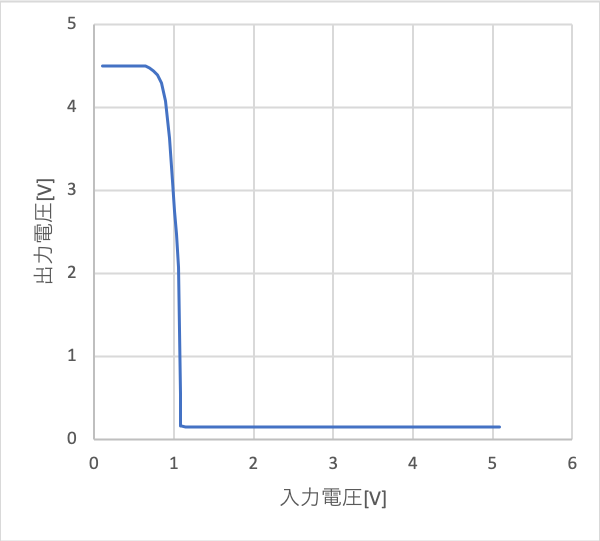
\includegraphics[width=0.8\linewidth]{fig1.png}
 \end{center}
 \caption{74LS04}
 \label{fig:1}
\end{figure}

\begin{figure}[htbp]
 \begin{center}
  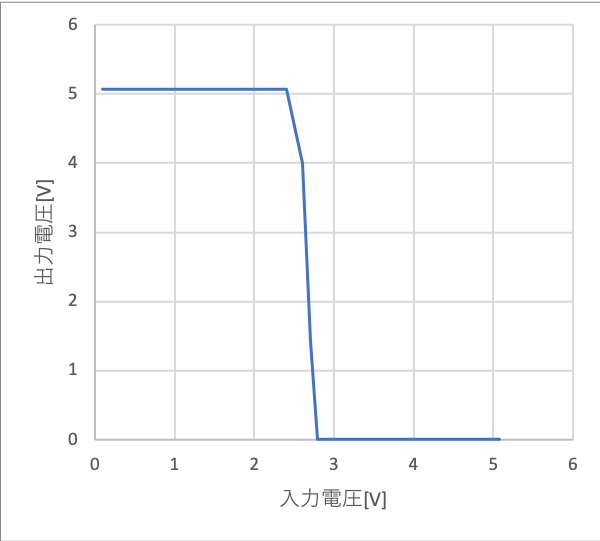
\includegraphics[width=0.7\linewidth]{fig2.png}
 \end{center}
 \caption{74HC04}
 \label{fig:2}
\end{figure}


\begin{figure}[htbp]
 \begin{center}
  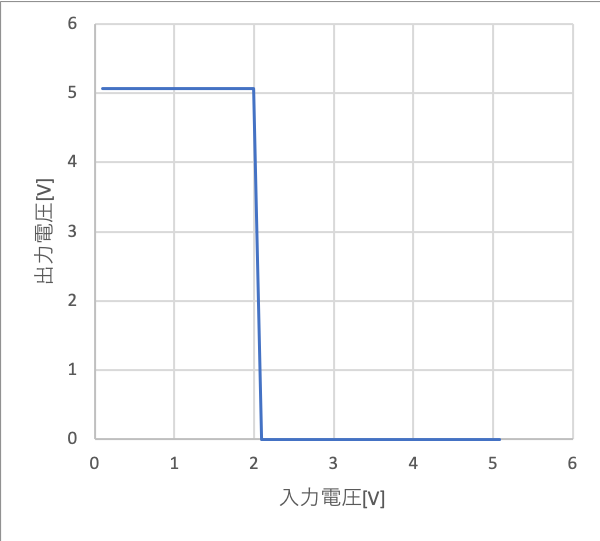
\includegraphics[width=0.7\linewidth]{fig3.png}
 \end{center}
 \caption{74HC14($V_{in}$下げていく)}
 \label{fig:3}
\end{figure}

\begin{figure}[htbp]
 \begin{center}
  \includegraphics[width=0.7\linewidth]{fig4.png}
 \end{center}
 \caption{74HC14($V_{in}$上げていく)}
 \label{fig:4}
\end{figure}

\subsection{Discussion}
今回はどのICについても入力電圧が5V付近の時出力電圧は0V付近を示し,逆に入力電圧が0付近の時出力電圧は5V付近を示したのでNOTゲートが正しく機能したと推測できる.

またTTLにおけるNOTゲートの動作を考察する.
\begin{figure}[htbp]
 \begin{center}
  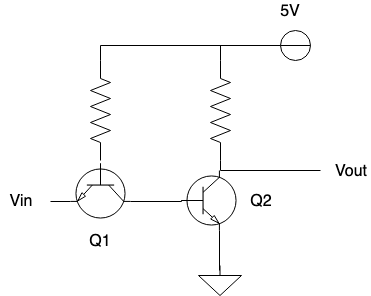
\includegraphics[width=0.7\linewidth]{fig6.png}
 \end{center}
 \caption{TTL NOTgate}
 \label{fig:6}
\end{figure}

TTLにおけるNOTゲートは図\ref{fig:6}のように表せる.
この回路において入力電圧$V_{in}$が0Vの時トランジスタQ1にいおいてベースエミッタ電圧$V{BE}$はスイッチング電圧である0.6Vを超えるためQ1は作動する.
この時Q2において$V_{BE}$は0VとなるためQ2は作動せず抵抗による電圧降下が起こらないため出力電が5Vとなると考えられる.

一方,入力電圧$V_{in}$が5V付近の時Q1において$V_{BE}$は逆バイアスとなりベースエミッタ間には電流は流れなくなる.
この時ベースコレクタ間に電流が流れることとなりトランジスタQ2は作動し抵抗により電圧降下を起こすこととなる.
したがって$V_{out}$は0Vを示すと考えられる.

次にCMOSにおけるNOTゲートの動作を考察する.
\begin{figure}[htbp]
 \begin{center}
  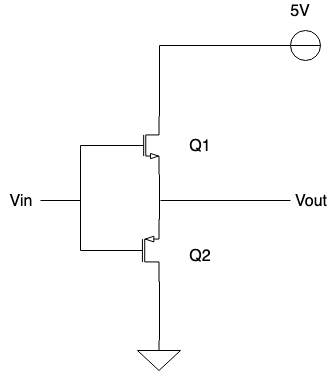
\includegraphics[width=0.7\linewidth]{fig7.png}
 \end{center}
 \caption{TTL NOTgate}
 \label{fig:7}
\end{figure}

図\ref{fig:7}のCOMOS回路ではpチャネル型(Q1)とnチャネル型(Q2)の二つのMOSFETを組み合わせて作られている.
それぞれ入力電圧$V_{in}$が0V付近の時はQ1がオンとなり出力電圧$V_{out}$は5Vとなり,入力電圧$V_{in}$が5V付近の時Q2がオンとなり出力電圧$V_{out}$は0V付近になることが予想される.

以上の考察から74LS04を用いた回路が他の三つのICを用いた回路よりも入出力電圧のグラフが緩やかであったのはトランジスタにおいてスイッチング電圧を境目として完全に電流が流れる流れないの関係が成り立つのではなく,スイッチング電圧の付近で少しずつ電流が流れ始めるためであると予想できる.

またCMOS回路においては回路内部で入力電圧によって選択的にスイッチのようにon,offのように作動するのでトランジスタを用いたTTL回路に比べて鋭い入出力電圧のグラフが得られたと考えられる.

% ヒステリシスの考察





%=============================================================
\newpage
\end{document}
